
\section{Neuartige Antriebe}
\label{s:Neartige Antriebe}
Obwohl sich der Kraftstoffverbrauch in der letzten 30 Jahren halbiert \cite{mensen2013handbuch} hat, bleiben die Auswirkungen hoch.
Bei der Untersuchung von alternativen Antrieben sind bestimmte Überlegungen relevant. Die Dichte des Energieträgers, Kosten 
und Verfügbarkeit des Rohstoffs, Sicherheit in Bezug auf Herstellung und Nutzung sowie direkte und indirekte \ce{CO2} Emissionen \cite{ansell2023review}.

In diesem Kapitel werden folgende vielversprechende Energieträger betrachtet und zusammengefasst: nachhaltige Kraftstoffe (SAF), 
Batterie-Antriebe (elektrochemische) und Wasserstoff.

\subsection{Sustainable Aviation Fuel (SAF)}

Sustainable Aviation Fuel oder nachhaltige Flugtreibstoffe sind synthetische flüssige Biotreibstoffe oder erneuerbare nicht biogene Stoffe, %(renewable non-biological sources), 
die mit herkömmlichen Flugkraftstoffen und bestehenden Betankungssystemen kompatibel sind.
Deswegen werden sie auch als Drop-In Treibstoffe bezeichnet \cite{iata_saf_2024}. 
Die SAFs werden zu herkömmlichen Treibstoffen beigemischt. IATA besagt, dass die zulässige Mischrate 
zurzeit bei max. 50 \% liegt. Es existieren bis jetzt elf Verfahrenswege aus unterschiedlichen Rohstoffen für die SAF-Produktion,
manche werden aktuell für die Nutzung bewertet \cite{icao_saf_conversion_2024}.

Die SAFs haben ähnliche Charakteristiken wie Kerosin, was bspw. die Energiedichte betrifft. Dennoch weist ein Großteil des SAF keine Aromaten auf. % Armaten oder Armoate?
Fehlende aromatische Verbindungen im SAF kann zu Leckagen in der Dichtung führen \cite{jarin2024emissions}. 
Aus diesem Grund ist bis jetzt kein Flugzeug für das Fliegen mit reinem SAF zertifiziert \cite{iata_saf_2024}.

Im Hinblick auf die Zukunft ist zu erwarten, dass die \ce{CO2}-Reduktion mit dem reinen SAF realisiert werden kann.
Ein praxisnahes Beispiel dafür war der erste transatlantische Demonstrationsflug im November 2023, durchgeführt von der Fluggesellschaft Virgin Atlantic,
welcher mit 100 \% SAF durchgeführt wurde \cite{virginatlantic_saf_2023}. 
%(davon 88 \%HEFA und 12\% Synthetic Aromatic Kerosene (SAK))
SAF Produktion erreichte im Jahr 2024 1 Million Tonnen \cite{iata2024}. Der Verbrauch der Luftverkehr, wie beschrieben oben
erreichte im Jahr 2023 92 Milliarden Gallonen, das bedeutet, dass SAF würde nur 0,8 \% der Gesamtverbrauch decken können

Es gibt keinen SAF-Flugtreibstoff, der Emissionen komplett vermeidet. 
Laut IATA durch Drop-In SAF können die Emissionen um 62 \% reduziert werden.
Jedoch durch bestimmte Verfahren können sie jedoch bis zu 95 \% reduziert werden \cite{icao_saf_conversion_2024}.

% "Current engine and propulsion systems are not compatible with 100 \% bio-jet 
%fuels which require retrofitting and development of new engine propulsion systems. "

%Die vier wichtigsten Technologie sind Hydroprocessed Esters and Fatty Acids (HEFA), Fischer-Tropsch (FT), Alcohol to Jet (ATJ) 
%und Power to Liquid (PtL). 
 
Aufgrund der kommerziellen Verfügbarkeit ist Hydroprocessed Esters and Fatty Acids (HEFA) eines der wichtigsten Verfahren.
Die HEFA wird aus tierischen und pflanzlichen Ölen und Fetten mittels Hydroprocessing hergestellt \cite{bauen2020sustainable}. 
Die Haupteinschränkung von HEFA ist die begrenzte Anzahl an Rohstoffen \cite{bauen2020sustainable}.
Power-to-liquid (PtL) ist ein weiteres potenzialreiches Verfahren.
Dieses katalytische Verfahren, nach Fischer-Tropsch, nutzt zur Herstellung eine Kombination aus 
Kohlenmonoxid \ce{CO} und durch Elektrolyse produzierten Wasserstoff \ce{H2} \cite{bauen2020sustainable}.
Das Verfahren erzeugt die höchsten \ce{CO2}-Emissionseinsparungen \cite{de2017life}, jedoch befindet es sich in einem früheren Stadium \cite{bauen2020sustainable}.
Eine zusätzliche Beschränkung besteht die Preise für SAF. In der Abbildung \ref{safpreis} sind Vergleichswerte für verschiedenen SAF 
und konventionelle Treibstoffe, als auch Vorhersagewerte dargestellt.
Dabei hat die HEFA die günstigsten Preise im Vergleich zu den Alternativen, dagegen die nachhaltigere PtL wird deutlich über 
den Preis von marktüblichen Treibstoffen hinausgehen.

\begin{figure}[h]
	\centering
	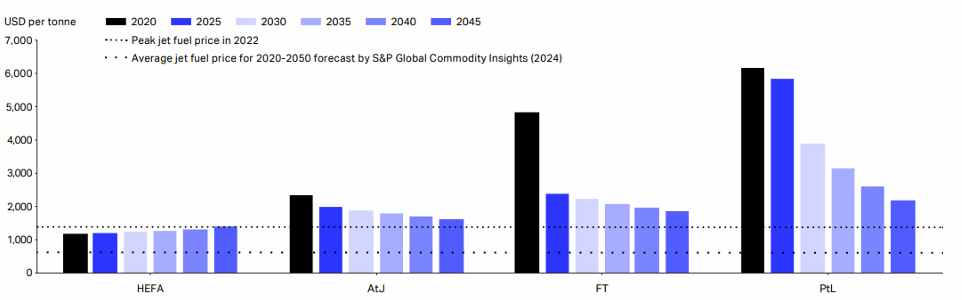
\includegraphics[width=0.8\linewidth]{Bilder/Preise SAF.png}
	\caption[Durchschnittlicher IATA-Mindestverkaufspreis (MSP) der wichtigsten SAF-Pfade über den Zeitraum 2020 bis 2050]{Durchschnittlicher IATA-Mindestverkaufspreis \cite{icao_saf_conversion_2024}}
	\label{safpreis}
\end{figure}
In Bezug auf die Infrastruktur sind manche davon überzeugt, dass keine Änderungen im Flugzeug oder am Betankungssystem notwendig sind \cite{sky2020hydrogen} %https://www.iata.org/en/pressroom/2023-releases/2023-06-04-03/.
Wobei Dahal et al. \cite{dahal2021techno} jedoch davon ausgeht, dass neue Antriebe und Triebwerke für die Nutzung des reinen SAF entwickelt werden müssen.
Das reine SAF wurde noch nicht zertifiziert, um in das Treibstofflager vom Flughafen zu gelangen \cite{iata_saf_2024}.


%In der Abbildung XX sind die SAF Produktionswege aus unterschiedlichen Quellen aufgelistet und den Teil des Kohlenstoffdioxids,
%die mit diesen Wegen reduziert werden. Bemerkenswert ist, dass die Herstellung
%aus einer Kombination aus Kohlenmonoxid (CO) und Wasserstoff (H2) durch das katalytische Verfahren nach Fischer-Tropsch (existing renewables), 
%auch PtL genannt, fast bis 100 \% CO2-Ausstoß reduziert, gefolgt von Municipal Solid Waste (MSW). 
%
%PtL: brauche ich das überhaupt?
%CO2 kann durch Direct Air Capture (DAC) aus der Luft gewonnen werden und dann mittels 
%Reverse-Water-Gas-Shift-Reaktion (RWGS) mit Wasserstoff zu CO2 umgewandelt werden. 
%PtL ist sehr energieintensiv und braucht erneuerbare Stromquelle (hängt davon ab).
%\cite{ansell2023review}
%Eine Herausforderung im Blick auf Ressourcen- und Flächenbedarf bleibt bei biogenen oder PtL-Synthese \cite{ansell2023review}.
%
%MSW ist Abfall aus nicht biogenen Quellen, wie Kunststoffe. \cite{icao_saf_conversion_2024} PtL SAF "Trotz der erheblichen Herausforderungen 
%bietet sich PtL SAF an, langfristig einer der stärksten Beiträge zur Energiewende der Fluggesellschaften zu werden."
%
%Kosten:
%https://www.icao.int/environmental-protection/Pages/SAF_RULESOFTHUMB.aspx
%https://theicct.org/sites/default/files/publications/Alternative_jet_fuels_cost_EU_20190320_1.pdf
%"Overall, estimates of capital spending on renewable diesel/HEFA facilities
%ra n g e f ro m a ro u n d € 0. 4 0 to €1.50 per liter of annual capacity, averaging around €0.60 per liter,
%with larger facilities generally having lower per-liter capital costs due to economies of scale"
%ICAO hat eine Reihe von Heuristiken rausgebracht, um Preisschätzungen unter SAF-Kraftstoffen zu ermitteln. (für USA)
%FT mit Feedstock CO2 from Direct Air Capture, H2 - Feedstock Price \$300/t, \$6/kg, Total capacity 1000 mill L/year.
%FT aus MSW - \$30/ton 
%
%
%Im März 2024 hat International Aero Engines AG (IAE) bei der MTU Maintenance ein V2500-Triebwerk mit 100 \% nachhaltigem 
%Flugkraftstoff HEFA-SPK getestet.
%
%Einbindung in Regularien
In EU-Richtlinien sowie in CORSIA sind die Kriterien für SAF-Qualität festgelegt.
Im Rahmen EU-ETS gelten SAF als emissionsfrei und bei der richtigen Zertifizierung sind vor der Abgabe von \ce{CO2}-Zertifikaten 
befreit \cite{icao_saf_conversion_2024}. Die Preise für nachhaltige Flugtreibstoffe sind zwei- bis zu fünfmal höher als für herkömmliche Kerosin \cite{iata_saf_2024} %unsicher wg Quelle.
Um Fluggesellschaften für die Nutzung der nachhaltigen Kraftstoffe zu motivieren, hat EU-ETS
20 Mio. Zertifikaten zur Verfügung gestellt \cite{icao_saf_conversion_2024}. 
In ReFuelEU sind vor allem die verpflichtete Beimischungsanteile von nachhaltigen Stoffen festgelegt.


%Nach ASTM D7566 müssen Kraftstoffe einen bestimmten Gehalt an Aromaten aufweisen, um kompatibel mit ben bestehenden Flugzeugen zu sein. (Quelle?)

%Quelle: Synthetic aromatic kerosene property prediction improvements with isomer specific characterization via GCxGC 
%and vacuum ultraviolet spectroscopy: 
%SAK besteht grundlegend aus Aromaten und unterscheidet sich deutlich von den anderen SAFs und wird für Aufschwellung von Dichtungen. 
%"Aromaten sind organische Verbindungen, die die Schmierfähigkeit, Dichte und Materialverträglichkeit des Flugkraftstoffs verbessern"
%Derzeit wird von ASTM evaluiert \cite{icao_saf_conversion_2024}.
%HEFA und SAK Mischung können die 100\% SAF-Flüge ermöglichen, dabei reduziert die Mischung die Rußpartikeln.

%Laut IATA durch Drop-In SAF können die Emissionen um 62 \% reduziert werden. https://www.iata.org/en/pressroom/2023-releases/2023-06-04-03/
%"As a drop-in solution, SAF is expected to deliver about 62\% of carbon mitigation needed to achieve net zero by 2050"
%
%Manche berichten, dass Flugdistanz bei SAF gleich(Quelle), und dazu zum Schluss gekommen, dass 
%Treibstoffverbrauch verringert werden kann(Quelle).
%Annahme: Verbrauch bei konventionellen und SAF gleich
